\section{Annex}
\label{sec-annex}

\subsection{Neuron and neural activity}
\label{subsec-neuron}

To further understand how brain activity works we first need to study a single neuron and its purpose. A neuron is an electrically excitable cell that has the function to communicate with other cells. It does it by nearly touching other cells called synapsis, transmits the message through its axon and delivers the message by synapsis\cite{Synapse} to another cell. Neurons are typically classified into types based on their function:
\\
\begin{itemize}
  \item Sensory neurons\cite{Sensoryneuron}: Which respond to stimuli of the sensory organs and send the signals to the spinal cord or brain.
  \item Motor neurons\cite{Motorneuron}: Its axons originate in the brain and spinal cord and innervate the muscles to produce muscle movements.
  \item Projection fiber\cite{Projectionfiber}: Are neurons found in the central nervous system and only establish synapses with other neurons, these consist of efferent and afferent fibers uniting the cortex with the lower parts of the brain and with the spinal cord.
  \item Interneuron\cite{Interneuron}: Is a neuron of the central nervous system, usually small and with a short axon, that interconnects with other neurons, but never with sensory receptors or muscle fibres, allowing it to perform more complex functions.
\end{itemize}
\leavevmode\\
Neurons transmit electrical waves originating from a transient change of permeability in the plasma membrane. Their propagation is due to the existence of a potential difference that arises due to different concentrations of ions on either side of the membrane, as described by the Nernst potential, between the inner and outer part of the cell (typically -70 mV). For the transmission of nervous impulses to other neurons, these do it by synapse, being a structure to pass electrical or chemical signals to another neuron or effector cell, there are two types of synapses\cite{Synapse}:
\\
\begin{itemize}
  \item	Chemical synapse: Electrical activity in the presynaptic neuron is converted into the release of a neurotransmitter that binds to the receptors located in the plasma membrane of the postsynaptic cell.
  \item	Electrical synapse: Is one in which transmission between the first neuron and the second is not by the secretion of a neurotransmitter, but by the passage of ions from one cell to another through gap junctions, small channels formed by the coupling of protein complexes, based on connexins, in closely adherent cells.
\end{itemize}

\leavevmode\\
These electrochemical processes when large numbers of neurons show synchronized activity, electric fields that they generate can be large enough to be detected outside the skull, and so using electroencephalography (EEG) or magnetoencephalography (MEG) brain activity can be recorded.
\\

\subsection{Structure}
\label{subsec-structure}
\leavevmode\\
Now that we know where brain activity originates from, we can further study how the brain structures. There are many parts in the brain, but for now we are going to focus on the cerebrum because it initiates and coordinates movement, regulates temperatures, speech, judgement, reasoning, problem-solving, emotions, learning…
\\
The cerebrum\cite{Cerebrum}, it’s the largest part of the brain, it’s divided by the medial longitudinal fissure in two hemispheres, each of these hemispheres has an outer layer of grey matter, the cerebral cortex and an inner layer of white matter. The fact that these are separated gives the opportunity for lateralisation of brain functions, which is the tendency of neurological functions to specialise in one hemisphere or the other, but even though the cerebrum\cite{Cerebrum} is separated, these are connected by the corpus callosum.
\\
\\
The cortex is mapped into fifty different functional areas known as Brodmann’s areas\cite{Brodmannarea}, defined by its cytoarchitecture (cellular composition), or histological structure and organization of cells. One scheme widely used (from Korbinian Brodmann)\cite{Brodmannarea} splits the cortex into 52 different numbered areas of different cellular structure and different functions.
\\
\begin{figure}[h]
  \caption{Brodmann areas by colors}
  \centering
  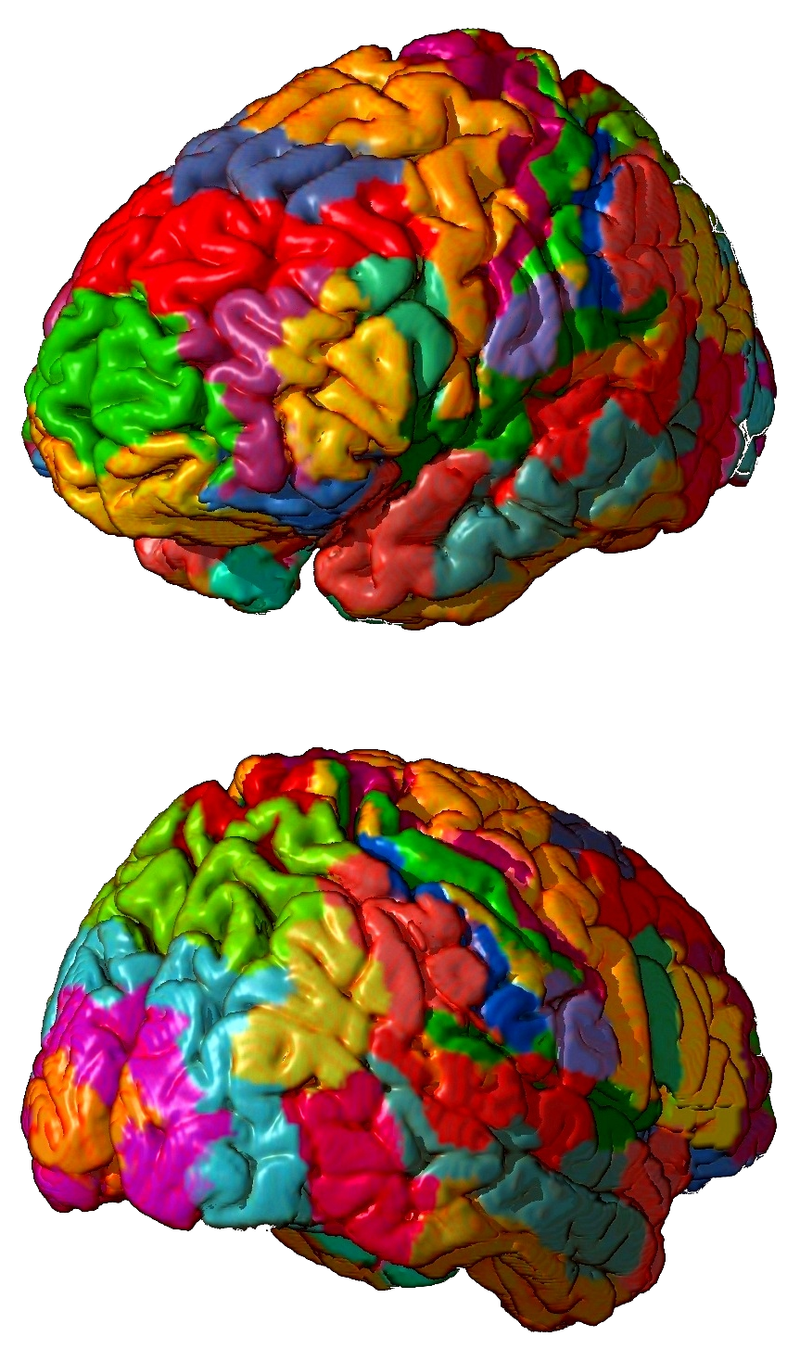
\includegraphics[width=4cm]{img/Brodmann_areas.png}
\end{figure}


Having clarified this brain structure, obtaining data with electrodes from brain activity, positioning of these is something to keep in touch with depending on what it’s being studied. The same goes for defining the dataset train and test data, to feed as input to the deep learning algorithm, opening a new field on how to treat and subdivide data to make the most of it.
\\